\documentclass{standalone}
\usepackage{pgfplots,pgfplotstable}
\begin{document}
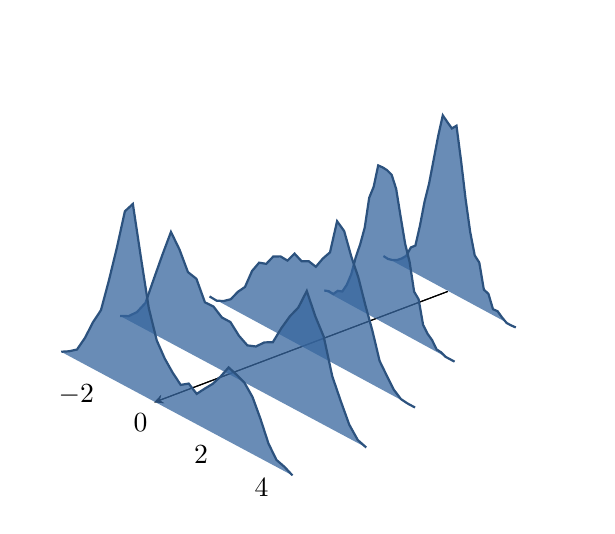
\begin{tikzpicture}

\definecolor{darkgreen}{RGB}{31,182,83}
\definecolor{darkblue}{RGB}{55,102,158}

\pgfplotstableread{
plot1   plot2   plot3   plot4
0       0       0       0
3.466   2.058   0       0
4.262   2.976   0.001   0
3.822   3.168   0.006   0.008
2.953   2.936   0.019   0.063
2.065   2.492   0.046   0.265
1.332   1.977   0.092   0.734
0.797   1.478   0.164   1.508
0.443   1.045   0.268   2.44
0.228   0.698   0.412   3.219
0.107   0.438   0.598   3.524
0.046   0.256   0.831   3.219
0.017   0.138   1.109   2.44
0.006   0.067   1.429   1.508
0.002   0.029   1.78    0.734
0       0.01    2.141   0.265
0       0.003   2.479   0.063
0       0.001   2.736   0.008
0       0       2.808   0
0       0       2.465   0
0       0       0       0
}\dummydata

\begin{axis}[
    view={50}{40},
    samples=30,
    domain=-4:4,
    samples y=0, ytick={1,...,4},
    zmin=0,
    y dir=reverse,
    yticklabels={,,},
    zticklabels={,,},
    ytick style={draw=none},
    ztick style={draw=none},
    xtick style={draw=none},
    z axis line style={draw opacity=0},
    x axis line style={draw opacity=0},
    axis y line = middle,
    area plot/.style={
        fill opacity=0.75,
        %draw=orange!80!black,thick,
        %fill=orange,
        %draw=darkgreen!80!black,thick,
        %fill=darkgreen,
        draw=darkblue!80!black,thick,
        fill=darkblue,
        mark=none,
    }
]
\addplot3 [area plot] coordinates {(-2.1255191731452943, 0, 2.0)(-1.9748047614097595, 0, 1.0)(-1.8240903496742247, 0, 4.0)(-1.67337593793869, 0, 10.0)(-1.5226615262031555, 0, 19.0)(-1.3719471144676207, 0, 31.0)(-1.2212327027320862, 0, 56.0)(-1.0705182909965516, 0, 66.0)(-0.9198038792610169, 0, 118.0)(-0.7690894675254822, 0, 179.0)(-0.6183750557899476, 0, 227.0)(-0.467660644054413, 0, 288.0)(-0.3169462323188783, 0, 349.0)(-0.16623182058334351, 0, 402.0)(-0.015517408847808944, 0, 392.0)(0.13519700288772563, 0, 383.0)(0.2859114146232604, 0, 395.0)(0.436625826358795, 0, 320.0)(0.5873402380943296, 0, 236.0)(0.7380546498298644, 0, 166.0)(0.8887690615653989, 0, 117.0)(1.0394834733009335, 0, 106.0)(1.1901978850364683, 0, 49.0)(1.3409122967720029, 0, 45.0)(1.4916267085075374, 0, 15.0)(1.6423411202430722, 0, 16.0)(1.7930555319786068, 0, 7.0)(1.9437699437141416, 0, 0.0)(2.0944843554496764, 0, 0.0)(2.2451987671852107, 0, 1.0)};

\addplot3 [area plot] coordinates {(-1.6571586632728574, 1, 4.0)(-1.5088122439384457, 1, 8.0)(-1.3604658246040344, 1, 7.0)(-1.2121194052696227, 1, 20.0)(-1.063772985935211, 1, 24.0)(-0.9154265666007995, 1, 45.0)(-0.7670801472663878, 1, 75.0)(-0.6187337279319762, 1, 120.0)(-0.4703873085975645, 1, 156.0)(-0.3220408892631529, 1, 200.0)(-0.17369446992874138, 1, 275.0)(-0.025348050594329763, 1, 306.0)(0.12299836874008196, 1, 361.0)(0.27134478807449347, 1, 362.0)(0.419691207408905, 1, 361.0)(0.5680376267433167, 1, 356.0)(0.7163840460777284, 1, 329.0)(0.8647304654121402, 1, 270.0)(1.0130768847465517, 1, 213.0)(1.1614233040809632, 1, 176.0)(1.309769723415375, 1, 113.0)(1.4581161427497864, 1, 101.0)(1.606462562084198, 1, 47.0)(1.7548089814186096, 1, 32.0)(1.9031554007530214, 1, 23.0)(2.051501820087433, 1, 7.0)(2.199848239421845, 1, 6.0)(2.348194658756256, 1, 1.0)(2.4965410780906674, 1, 1.0)(2.644887497425079, 1, 1.0)};

\addplot3 [area plot] coordinates {(-3.023305811882019, 2, 3.0)(-2.7893237543106078, 2, 2.0)(-2.5553416967391964, 2, 10.0)(-2.3213596391677855, 2, 23.0)(-2.0873775815963747, 2, 49.0)(-1.8533955240249633, 2, 69.0)(-1.619413466453552, 2, 115.0)(-1.3854314088821411, 2, 143.0)(-1.1514493513107298, 2, 149.0)(-0.9174672937393187, 2, 175.0)(-0.6834852361679076, 2, 184.0)(-0.44950317859649647, 2, 183.0)(-0.21552112102508536, 2, 208.0)(0.018460936546325746, 2, 199.0)(0.25244299411773685, 2, 208.0)(0.48642505168914796, 2, 204.0)(0.7204071092605593, 2, 232.0)(0.9543891668319704, 2, 255.0)(1.1883712244033813, 2, 336.0)(1.4223532819747926, 2, 322.0)(1.656335339546204, 2, 272.0)(1.8903173971176148, 2, 232.0)(2.1242994546890257, 2, 176.0)(2.358281512260437, 2, 125.0)(2.5922635698318484, 2, 65.0)(2.8262456274032592, 2, 40.0)(3.0602276849746706, 2, 16.0)(3.294209742546082, 2, 3.0)(3.528191800117493, 2, 1.0)(3.7621738576889037, 2, 1.0)};

\addplot3 [area plot] coordinates {(-3.5572386503219606, 3, 2.0)(-3.2768911600112913, 3, 12.0)(-2.996543669700622, 3, 32.0)(-2.7161961793899536, 3, 64.0)(-2.4358486890792843, 3, 131.0)(-2.155501198768616, 3, 197.0)(-1.8751537084579466, 3, 260.0)(-1.5948062181472775, 3, 230.0)(-1.3144587278366087, 3, 188.0)(-1.0341112375259398, 3, 183.0)(-0.7537637472152707, 3, 139.0)(-0.47341625690460165, 3, 140.0)(-0.1930687665939328, 3, 125.0)(0.08727872371673628, 3, 125.0)(0.36762621402740514, 3, 104.0)(0.647973704338074, 3, 92.0)(0.9283211946487433, 3, 100.0)(1.2086686849594122, 3, 120.0)(1.489016175270081, 3, 131.0)(1.7693636655807499, 3, 174.0)(2.0497111558914187, 3, 212.0)(2.330058646202088, 3, 243.0)(2.610406136512757, 3, 292.0)(2.8907536268234257, 3, 244.0)(3.171101117134095, 3, 207.0)(3.451448607444764, 3, 126.0)(3.7317960977554328, 3, 79.0)(4.012143588066102, 3, 35.0)(4.292491078376771, 3, 10.0)(4.572838568687439, 3, 3.0)};

\addplot3 [area plot] coordinates {(-3.082342638969421, 4, 1.0)(-2.8188495111465453, 4, 12.0)(-2.5553563833236694, 4, 26.0)(-2.291863255500793, 4, 63.0)(-2.028370127677917, 4, 109.0)(-1.7648769998550413, 4, 147.0)(-1.5013838720321653, 4, 226.0)(-1.2378907442092895, 4, 312.0)(-0.9743976163864134, 4, 406.0)(-0.7109044885635374, 4, 433.0)(-0.44741136074066135, 4, 320.0)(-0.18391823291778553, 4, 211.0)(0.07957489490509051, 4, 146.0)(0.34306802272796655, 4, 114.0)(0.6065611505508426, 4, 91.0)(0.8700542783737186, 4, 73.0)(1.1335474061965947, 4, 86.0)(1.3970405340194705, 4, 72.0)(1.6605336618423463, 4, 94.0)(1.9240267896652226, 4, 115.0)(2.1875199174880984, 4, 142.0)(2.451013045310974, 4, 173.0)(2.7145061731338505, 4, 166.0)(2.9779993009567263, 4, 157.0)(3.241492428779602, 4, 134.0)(3.5049855566024783, 4, 93.0)(3.7684786844253546, 4, 46.0)(4.03197181224823, 4, 18.0)(4.295464940071106, 4, 12.0)(4.5589580678939825, 4, 2.0)};


%\pgfplotsinvokeforeach{4,3,...,1}{
%    %\addplot3 [area plot] table [x expr=\coordindex, y expr=#1, z=plot#1] {\dummydata};
%    \addplot3 [area plot] table [x expr=\coordindex, y expr=#1, z=plot#1] {\dummydata};
%}
\end{axis}
\end{tikzpicture}

\end{document}
